
\documentclass{beamer}
\usecolortheme{dove}
\setbeamertemplate{navigation symbols}{}
\usepackage{amsmath,amssymb,amsfonts,amsthm, multicol, subfigure, color}
\usepackage{bm}
\usepackage{graphicx}
\usepackage{tabularx}
\usepackage{booktabs}
\usepackage{hyperref}
\usepackage{pdfpages}
\usepackage{xcolor}
\definecolor{seagreen}{RGB}{46, 139, 87}
\def\independenT#1#2{\mathrel{\rlap{$#1#2$}\mkern2mu{#1#2}}}
\newcommand\indep{\protect\mathpalette{\protect\independenT}{\perp}}
\def\log{\text{log}}
\newcommand\logit{\text{logit}}
\newcommand\iid{\stackrel{\text{iid}}{\sim}}
\newcommand\E{\text{E}}
\newcommand\V{\text{V}}
\renewcommand\P{\text{P}}
\newcommand{\Cov}{\text{Cov}}
\newcommand{\Cor}{\text{Cor}}
\newcommand\doop{\texttt{do}}
\usepackage{stackrel}
\usepackage{tikz}
\usetikzlibrary{arrows,shapes.arrows,positioning,shapes,patterns,calc}
\newcommand\slideref[1]{\vskip .1cm \tiny \textcolor{gray}{{#1}}}
\newcommand\red[1]{\color{red}#1}
\newcommand\blue[1]{\color{blue}#1}
\newcommand\gray[1]{\color{gray}#1}
\newcommand\seagreen[1]{\color{seagreen}#1}
\newcommand\purple[1]{\color{purple}#1}
\newcommand\orange[1]{\color{orange}#1}
\newcommand\black[1]{\color{black}#1}
\newcommand\white[1]{\color{white}#1}
\newcommand\teal[1]{\color{teal}#1}
\newcommand\magenta[1]{\color{magenta}#1}
\newcommand\Fuchsia[1]{\color{Fuchsia}#1}
\newcommand\BlueGreen[1]{\color{BlueGreen}#1}
\newcommand\bblue[1]{\textcolor{blue}{\textbf{#1}}}
\newcommand\bred[1]{\textcolor{red}{\textbf{#1}}}
\newcommand\bgray[1]{\textcolor{gray}{\textbf{#1}}}
\newcommand\bgreen[1]{\textcolor{seagreen}{\textbf{#1}}}
\newcommand\bref[2]{\href{#1}{\color{blue}{#2}}}
\colorlet{lightgray}{gray!40}
\pgfdeclarelayer{bg}    % declare background layer for tikz
\pgfsetlayers{bg,main} % order layers for tikz
\newcommand\mycite[1]{\begin{scriptsize}\textcolor{darkgray}{(#1)}\end{scriptsize}}
\newcommand{\tcframe}{\frame{
%\small{
\only<1|handout:0>{\tableofcontents}
\only<2|handout:1>{\tableofcontents[currentsubsection]}}
%}
}

\usepackage[round]{natbib}
\bibliographystyle{humannat-mod}
\setbeamertemplate{enumerate items}[default]
\usepackage{mathtools}

\newcommand{\goalsframe}{\begin{frame}{Learning goals for today}
At the end of class, you will be able to:
\begin{enumerate}
\item Present treatments that unfold over time in DAGs
\item Recognize the difficulties of treatment-induced confounding
\end{enumerate} \vskip .2in
\end{frame}}

\title{15. Treatments in many time periods.\\The problem.}
\author{Ian Lundberg\\Cornell Info 6751: Causal Inference in Observational Settings\\Fall 2022}
\date{13 Oct 2022}

\begin{document}

\maketitle

\goalsframe

\begin{frame}{Treatments in many time periods: Motivation}
Suppose you teach second grade \pause
\begin{itemize}
\item Every month, you assess children's ability to sound out words \pause
\item You assign parent volunteers to read with those who struggle \pause
\item In December, you hope every child can read a picture book \pause
\end{itemize}
Task: Draw this in a DAG
\end{frame}

\begin{frame}{Treatments in many time periods: Motivation}

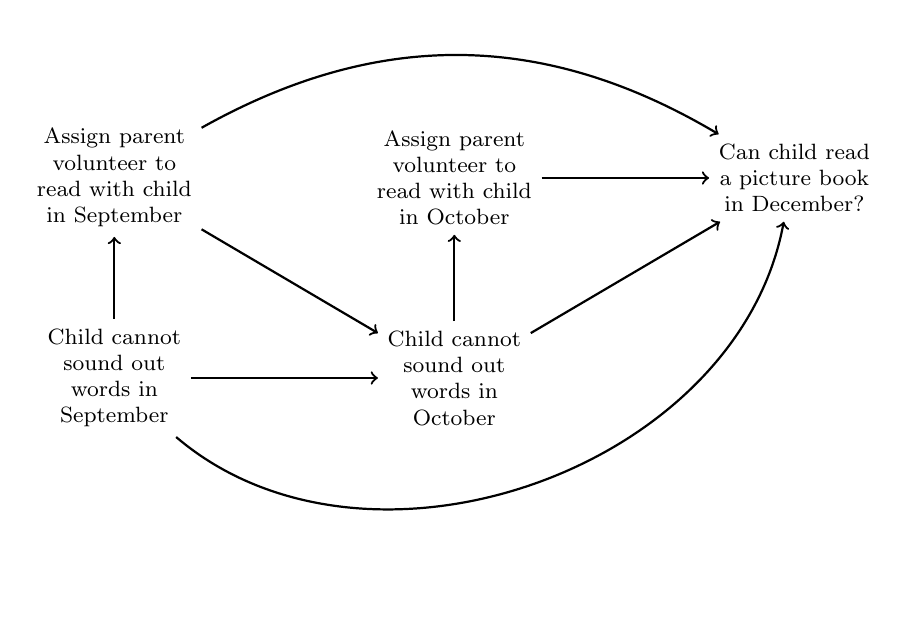
\begin{tikzpicture}[x = 1.7in, y = 1in]
\node[font = \footnotesize, align = center] (l0) at (0,-1) {Child cannot\\sound out\\words in\\September}; \pause
\node[font = \footnotesize, align = center] (a0) at (0,0) {Assign parent\\volunteer to\\read with child\\in September};
\draw[->, thick] (l0) -- (a0); \pause
\node[font = \footnotesize, align = center] (l1) at (1,-1) {Child cannot\\sound out\\words in\\October};
\draw[->, thick] (l0) -- (l1);
\draw[->, thick] (a0) -- (l1); \pause
\node[font = \footnotesize, align = center] (a1) at (1,0) {Assign parent\\volunteer to\\read with child\\in October};
\draw[->, thick] (l1) -- (a1); \pause
\node[font = \footnotesize, align = center] (y) at (2,0) {Can child read\\a picture book\\in December?};
\draw[->, thick] (l0) to[bend right = 60] (y);
\draw[->, thick] (a0) to[bend left] (y);
\draw[->, thick] (l1) -- (y);
\draw[->, thick] (a1) -- (y);
\end{tikzpicture}

\end{frame}

\begin{frame}{Treatments in many time periods: A general problem}

\begin{center}
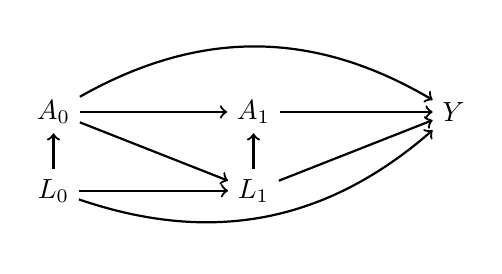
\begin{tikzpicture}[x = 1in]
\node (y) at (2,0) {$Y$};
\node (l0) at (0,-1) {$L_0$};
\node (a0) at (0,0) {$A_0$};
\draw[->, thick] (l0) -- (a0);
\draw[->, thick] (l0) to[bend right] (y);
\draw[->, thick] (a0) to[bend left] (y);
\node (l1) at (1,-1) {$L_1$};
\node (a1) at (1,0) {$A_1$};
\draw[->, thick] (a0) -- (a1);
\draw[->, thick] (l0) -- (l1);
\draw[->, thick] (a0) -- (l1);
\draw[->, thick] (l1) -- (a1);
\draw[->, thick] (l1) -- (y);
\draw[->, thick] (a1) -- (y);
\end{tikzpicture}
\end{center} \pause

This causal structure occurs
\begin{itemize}
\item when a policymaker targets treatment $A_k$ at time $k$ given confounders $L_k$ measured at that time
\item in observational settings where treatments unfold over time
\end{itemize} \vskip .1in \pause
Goal: Study the outcome $Y$ would be realized on average if $A_0,\dots,A_k$ are set to the values $a_0,\dots,a_k$.

\end{frame}

\begin{frame}{Treatments in many time periods:\\The curse of dimensionality}

\begin{center}
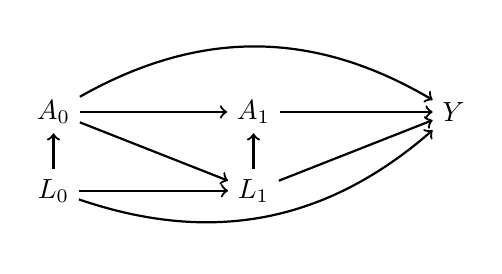
\begin{tikzpicture}[x = 1in]
\node (y) at (2,0) {$Y$};
\node (l0) at (0,-1) {$L_0$};
\node (a0) at (0,0) {$A_0$};
\draw[->, thick] (l0) -- (a0);
\draw[->, thick] (l0) to[bend right] (y);
\draw[->, thick] (a0) to[bend left] (y);
\node (l1) at (1,-1) {$L_1$};
\node (a1) at (1,0) {$A_1$};
\draw[->, thick] (a0) -- (a1);
\draw[->, thick] (l0) -- (l1);
\draw[->, thick] (a0) -- (l1);
\draw[->, thick] (l1) -- (a1);
\draw[->, thick] (l1) -- (y);
\draw[->, thick] (a1) -- (y);
\end{tikzpicture}
\end{center}
 \vskip .2in
Each $A_k$ is binary. How many potential outcomes are there? \pause
\begin{itemize}
\item $\bar{a} = (0,0)$: No reading with a parent
\item $\bar{a} = (1,0)$: Read in September, not October
\item $\bar{a} = (0,1)$: Read in October, not September
\item $\bar{a} = (1,1)$: Always read with a parent
\end{itemize}

\end{frame}

\begin{frame}{Treatments in many time periods:\\The curse of dimensionality}

Suppose the teacher can assign (or not) a parent volunteer to read with a child in each of 9 months in the school year
$$A_0,\dots,A_8$$ \pause
There are then $2^9 = 512$ potential outcomes $Y^{a_0,\dots,a_8}$ for each child \vskip .4in \pause
This is why we focus on \bblue{treatment strategies}

\end{frame}

\begin{frame}{Treatment strategy}

A treatment strategy is a counterfactual policy rule $g()$ for assigning the treatment \vskip .2in \pause

\bgray{Example:}\\
Assign a parent volunteer to read with a child whenever the child struggles sounding out words \pause

$$g(L_k) = \mathbb{I}(L_k = 0)$$ \pause

We would then assign treatment $A_k = g(L_k)$ \vskip .2in \pause
This involves \bblue{many treatments}, but only \bblue{one strategy}.

\end{frame}

\begin{frame}{Treatment strategy: Exercise}

Use math to define the following strategy: \vskip .3in

Assign a parent volunteer to read with a child $A_k = 1$ if and only if the child struggles sounding out words $L_k=0$ and the child did not receive this support last month $A_{k-1}=0$ \pause

$$g(L_k, A_{k-1}) = \mathbb{I}(L_k = 0, A_{k-1} = 0)$$

\end{frame}

\begin{frame}{Treatment strategy: Static and dynamic}

\pause
A \bblue{static} strategy assigns treatments in advance
\begin{itemize}
\item Example: Always treat. $g() = 1$
\end{itemize} \vskip .2in \pause
A \bblue{dynamic} strategy assigns treatments as a function of the changing values of confounding variables
\begin{itemize}
\item Example: Treat if has difficulty sounding out words. $g(L_k) = \mathbb{I}(L_k = 0)$
\end{itemize}
\end{frame}

\begin{frame}[t]{Identification: The adjustment set} \pause
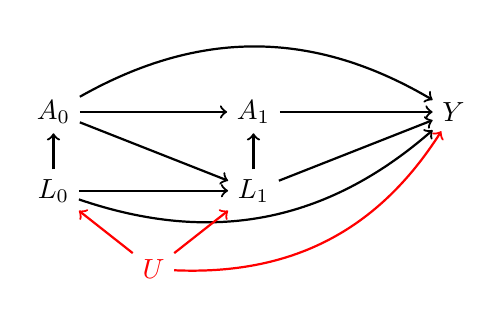
\begin{tikzpicture}[x = 1in]
\node (y) at (2,0) {$Y$};
\node[red] (u) at (.5,-2) {$U$};
\node (l0) at (0,-1) {$L_0$};
\node (a0) at (0,0) {$A_0$};
\draw[->, thick] (l0) -- (a0);
\draw[->, thick] (l0) to[bend right] (y);
\draw[->, thick] (a0) to[bend left] (y);
\node (l1) at (1,-1) {$L_1$};
\node (a1) at (1,0) {$A_1$};
\draw[->, thick] (a0) -- (a1);
\draw[->, thick] (l0) -- (l1);
\draw[->, thick] (a0) -- (l1);
\draw[->, thick] (l1) -- (a1);
\draw[->, thick] (l1) -- (y);
\draw[->, thick] (a1) -- (y);
\draw[->, thick, red] (u) -- (l0);
\draw[->, thick, red] (u) -- (l1);
\draw[->, thick, red] (u) to[bend right] (y);
\end{tikzpicture} \vskip .2in
\begin{enumerate} \pause
\item What is the sufficient adjustment set to identify \pause
\begin{enumerate}[a)]
\item The total effect of $A_0$ on $Y$ \pause
\item The total effect of $A_1$ on $Y$ \pause
\end{enumerate}
\item We want to identify the effect of $\bar{A} = (A_0,A_1)$ on $Y$\\\pause Can we jointly block all backdoor paths between $\bar{A}$ and $Y$? \pause
\end{enumerate} \vskip .2in
$U$ is unobserved and cannot be part of the adjustment set
\end{frame}

\begin{frame}[t]{Identification: The adjustment set}
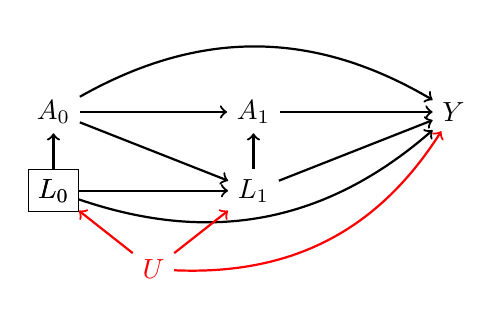
\begin{tikzpicture}[x = 1in]
\node (y) at (2,0) {$Y$};
\node[red] (u) at (.5,-2) {$U$};
\node<1> (l0) at (0,-1) {$L_0$};
\node<2>[draw] (l0) at (0,-1) {$L_0$};
\node (a0) at (0,0) {$A_0$};
\draw[->, thick] (l0) -- (a0);
\draw[->, thick] (l0) to[bend right] (y);
\draw[->, thick] (a0) to[bend left] (y);
\node (l1) at (1,-1) {$L_1$};
\node (a1) at (1,0) {$A_1$};
\draw[->, thick] (a0) -- (a1);
\draw[->, thick] (l0) -- (l1);
\draw[->, thick] (a0) -- (l1);
\draw[->, thick] (l1) -- (a1);
\draw[->, thick] (l1) -- (y);
\draw[->, thick] (a1) -- (y);
\draw[->, thick, red] (u) -- (l0);
\draw[->, thick, red] (u) -- (l1);
\draw[->, thick, red] (u) to[bend right] (y);
\end{tikzpicture} \vskip .2in
\begin{enumerate}
\item What is the sufficient adjustment set to identify
\begin{enumerate}[a)]
\item The total effect of $A_0$ on $Y$
\item \gray{The total effect of $A_1$ on $Y$}
\end{enumerate}
\item \gray{We want to identify the effect of $\bar{A} = (A_0,A_1)$ on $Y$\\Can we jointly block all backdoor paths between $\bar{A}$ and $Y$?}
\end{enumerate} \vskip .2in
\gray{$U$ is unobserved and cannot be part of the adjustment set}
\end{frame}

\begin{frame}[t]{Identification: The adjustment set}
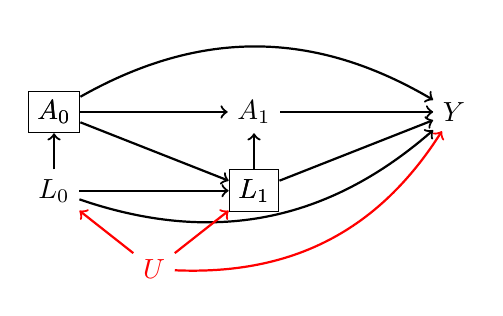
\begin{tikzpicture}[x = 1in]
\node (y) at (2,0) {$Y$};
\node[red] (u) at (.5,-2) {$U$};
\node (l0) at (0,-1) {$L_0$};
\node<1> (a0) at (0,0) {$A_0$};
\node<1> (l1) at (1,-1) {$L_1$};
\node<2>[draw] (a0) at (0,0) {$A_0$};
\node<2>[draw] (l1) at (1,-1) {$L_1$};
\draw[->, thick] (l0) -- (a0);
\draw[->, thick] (l0) to[bend right] (y);
\draw[->, thick] (a0) to[bend left] (y);
\node (a1) at (1,0) {$A_1$};
\draw[->, thick] (a0) -- (a1);
\draw[->, thick] (l0) -- (l1);
\draw[->, thick] (a0) -- (l1);
\draw[->, thick] (l1) -- (a1);
\draw[->, thick] (l1) -- (y);
\draw[->, thick] (a1) -- (y);
\draw[->, thick, red] (u) -- (l0);
\draw[->, thick, red] (u) -- (l1);
\draw[->, thick, red] (u) to[bend right] (y);
\end{tikzpicture} \vskip .2in
\begin{enumerate}
\item What is the sufficient adjustment set to identify
\begin{enumerate}[a)]
\item \gray{The total effect of $A_0$ on $Y$}
\item \black{The total effect of $A_1$ on $Y$}
\end{enumerate}
\item \gray{We want to identify the effect of $\bar{A} = (A_0,A_1)$ on $Y$\\Can we jointly block all backdoor paths between $\bar{A}$ and $Y$?}
\end{enumerate} \vskip .2in
\gray{$U$ is unobserved and cannot be part of the adjustment set}
\end{frame}

\begin{frame}[t]{Identification: The adjustment set}
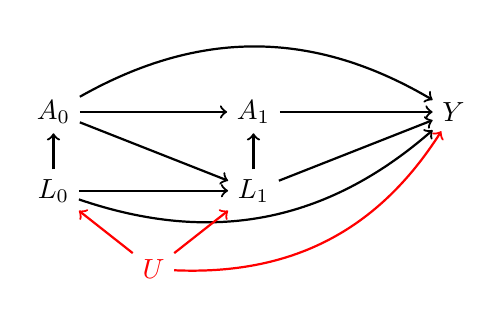
\begin{tikzpicture}[x = 1in]
\node (y) at (2,0) {$Y$};
\node[red] (u) at (.5,-2) {$U$};
\node (l0) at (0,-1) {$L_0$};
\node (a0) at (0,0) {$A_0$};
\node (l1) at (1,-1) {$L_1$};
\draw[->, thick] (l0) -- (a0);
\draw[->, thick] (l0) to[bend right] (y);
\draw[->, thick] (a0) to[bend left] (y);
\node (a1) at (1,0) {$A_1$};
\draw[->, thick] (a0) -- (a1);
\draw[->, thick] (l0) -- (l1);
\draw[->, thick] (a0) -- (l1);
\draw[->, thick] (l1) -- (a1);
\draw[->, thick] (l1) -- (y);
\draw[->, thick] (a1) -- (y);
\draw[->, thick, red] (u) -- (l0);
\draw[->, thick, red] (u) -- (l1);
\draw[->, thick, red] (u) to[bend right] (y);
\end{tikzpicture} \only<2>{\begin{large} \bblue{(2) has no solution!} \end{large}}\vskip .2in
\begin{enumerate}
\item \gray{What is the sufficient adjustment set to identify}
\begin{enumerate}[a)]
\item \gray{The total effect of $A_0$ on $Y$}
\item \gray{The total effect of $A_1$ on $Y$}
\end{enumerate}
\item \black{We want to identify the effect of $\bar{A} = (A_0,A_1)$ on $Y$\\Can we jointly block all backdoor paths between $\bar{A}$ and $Y$?}
\end{enumerate} \vskip .2in
\gray{$U$ is unobserved and cannot be part of the adjustment set}
\end{frame}

\begin{frame}[t]{Identification: The adjustment set}
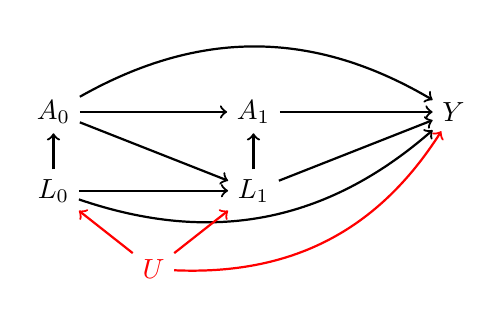
\begin{tikzpicture}[x = 1in]
\node (y) at (2,0) {$Y$};
\node[red] (u) at (.5,-2) {$U$};
\node (l0) at (0,-1) {$L_0$};
\node (a0) at (0,0) {$A_0$};
\node (l1) at (1,-1) {$L_1$};
\draw[->, thick] (l0) -- (a0);
\draw[->, thick] (l0) to[bend right] (y);
\draw[->, thick] (a0) to[bend left] (y);
\node (a1) at (1,0) {$A_1$};
\draw[->, thick] (a0) -- (a1);
\draw[->, thick] (l0) -- (l1);
\draw[->, thick] (a0) -- (l1);
\draw[->, thick] (l1) -- (a1);
\draw[->, thick] (l1) -- (y);
\draw[->, thick] (a1) -- (y);
\draw[->, thick, red] (u) -- (l0);
\draw[->, thick, red] (u) -- (l1);
\draw[->, thick, red] (u) to[bend right] (y);
\end{tikzpicture} \vskip .2in
A joint adjustment set for $\bar{A}$ is doomed \pause
\begin{itemize}
\item What happens if you adjust for $L_1$? \pause
\begin{itemize}
\item You block a causal path: $A_0\rightarrow \boxed{L_1}\rightarrow Y$
\item You open a backdoor path: $A_0 \rightarrow \boxed{L_1}\leftarrow U\rightarrow Y$
\end{itemize} \pause
\item What happens if you don't adjust for $L_1$? \pause
\begin{itemize}
\item A backdoor path remains: $A_1 \leftarrow L_1\rightarrow Y$
\end{itemize} 
\end{itemize} \pause
Next class: How to correctly adjust for treatment-induced confounding
\end{frame}

\goalsframe

\begin{frame}{Let me know what you are thinking}

\begin{huge} \bref{https://tinyurl.com/CausalQuestions}{tinyurl.com/CausalQuestions} \end{huge}
\vskip .7in

Office hours TTh 11am-12pm and at \bref{https://calendly.com/ianlundberg/office-hours}{calendly.com/ianlundberg/office-hours}\\Come say hi!

\end{frame}

\end{document}